%% 情報学群実験第3,4(C)用のレポートテンプレート
%
\documentclass[a4j,titlepage]{jarticle}
%% プリアンブルここから
\usepackage[dvipdfmx]{graphicx}
\usepackage{url}
\usepackage{comment}
\usepackage{here}
%
\title{\huge 配達支援システム\\
		内部設計書}
\author{第1版\\
        ONO-Systems\\}
\date{\today}

%本文
\begin{document}
\maketitle

%目次
\tableofcontents
\clearpage


\section{開発対象のシステム概要}
本システムは,配達物の配達支援を行うシステムです.主な機能を以下に示します.
\begin{itemize}
\item 消費者への通知機能\\
  配達物が届く際に,消費者の端末に配達物に関する通知を送ります.
  消費者はその際に,配達物を受け取れるかどうかを選択することができます.
  受け取ることができない場合は,配達日時を変更することが可能です.
\item 消費者の受取選択結果のリアルタイム表示機能\\
  消費者が選択した受取可否の情報を,配達員側の端末にリアルタイムに表示します.
  受け取る場合,受け取らない場合,未選択の場合を異なる色で表現し,受取選択結果の一覧を表示します.
\item 配達先の位置情報の表示機能\\
  配達員側の機能に,マップ画面で配達先の位置を表示する機能があります.
  受取可否ステータス別に表示でき,消費者が受け取らない選択をした配達物を非表示にする機能を実現します.
\item 配達物のソート機能\\
  配達員側では,配達物一覧を,現在位置と配達先間の距離順で並びかえる機能があります.
  また,配達物の指定時間順でソートする機能も実装します.
\end{itemize}


\section{開発環境}
本システムの開発環境を以下に示します.
\begin{itemize}
\item Android アプリケーション\\
  Android Studio ver3.0以上
\item サーバ\\
  AWS(AmazonWebService)
\item 開発言語\\
  Java,MySQL
\item 文書・コード管理\\
  GitHub
\item サービス\\
  Firebase,Google Maps API
\end{itemize}


\section{動作環境}
\begin{itemize}
\item Android アプリケーション\\
  APIレベル 24以上
\item サーバ\\
  AWS(AmazonWebService)
\end{itemize}


\section{コーディング規約}
本プロジェクトのプログラムは,以下の規則を遵守します.
\subsection{コンポーネントやクラスについて}
\begin{itemize}
\item UpperCamelCaseを利用する
\item Component名は最後につける(Activity,Fragment,TextAreaなど)
\item 本プロジェクトで頻繁に利用する名詞は以下の表を用いて命名する(表\ref{termTable}参照)
\begin{table}[htb]
\centering
\caption{本プロジェクトで利用する名詞の英単語表}
\label{termTable}
\begin{tabular}{|ll|}
\hline
内部設計書での名前 & 英単語      \\ \hline
アカウント保持者  & User     \\
消費者       & Customer \\
配達員       & Courier  \\
配達物       & Delivery \\ \hline
\end{tabular}
\end{table}
\end{itemize}

\subsection{変数の命名について}
\begin{itemize}
\item 命名には英語を用いる
\item 名前から役割が読み取れるように命名する
\item グローバル変数に用いる英単語は省略しない(String ⇒ Strなど)
\item LowerCamelCaseを利用する
\item 定数は全て大文字で表し,スネークケースで連結する
\item forやwhileのカウンタ変数には,i,j,kを用いる
\end{itemize}

\subsection{関数の命名について}
\begin{itemize}
\item 意味と英単語の対応付けを統一する(表\ref{namingTable})
\item 名前は動詞で始める
\item LowerCamelCaseを利用する
\begin{table}[htb]
\centering
\caption{命名に使う英単語表}
\label{namingTable}
\begin{tabular}{|lll|}
\hline
意味            & 英単語    & 例                    \\ \hline
真偽値を取得        & is     & \#isCreated          \\
値を代入          & set    & \#setDelivery        \\
引数を含むか判定      & has    & \#hasFragment        \\
特定の動作をしたときに動作 & on     & \#onClick            \\
新しく作る         & create & \#createSubActivity  \\
新しく作る         & new    & \#newDelivery        \\
更新            & update & \#updateDeliveryDate \\
サーバから情報を取得    & fetch  & \#fetchDeliveryList  \\ \hline
\end{tabular}
\end{table}
\end{itemize}

\subsection{コーディングについて}
\begin{itemize}
\item 字下げは半角スペース2つを用いる
\item マジックナンバーは使用しない
\item 安易にネット上のソースコードを利用しない
\item classやif,whileなどのブロック始点のブラケット('\{')は改行せずに,半角スペースを空けて記述する
\item 機能が完成したとき(Pull Requestsを出すとき)にデバッグ用のコードを残さない
\end{itemize}

\subsection{コメントについて}
\begin{itemize}
    \item 複雑な処理はコメントをつける
    \item メソッドにはコメントをつける
    \item TODO:など,コードの説明でないコメントはPullRequestsを出すときには消す
\end{itemize}

\section{ネットワーク設計}
本システムのネットワークは図\ref{fig:n_d}のように構成されます.

\begin{figure}[H]
 \begin{center}
  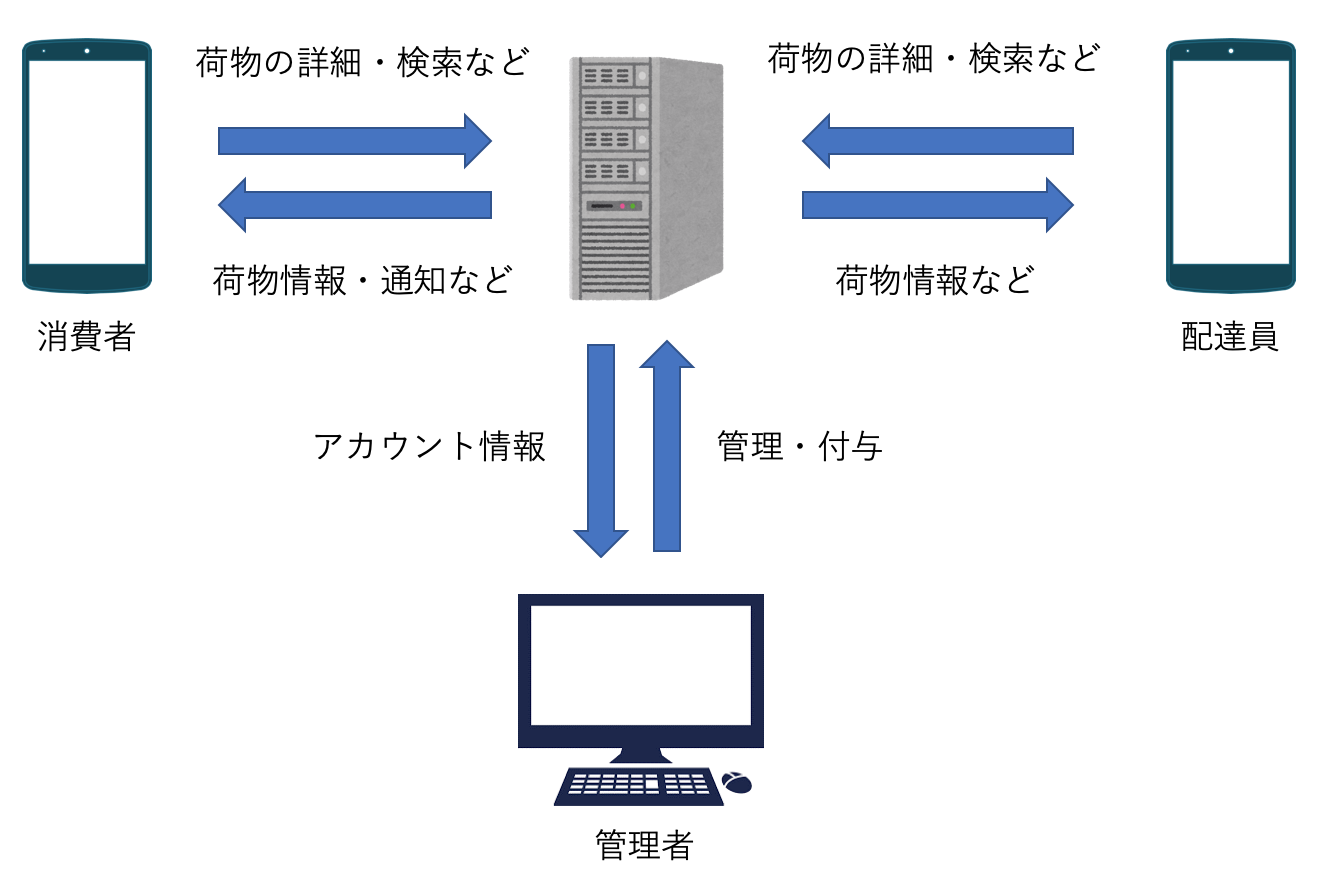
\includegraphics[width=140mm]{Network_Diagram.png}
  \caption{ネットワーク構成図}
  \label{fig:n_d}
 \end{center}

\end{figure}

\section{Android モジュール設計}
Androidのモジュール設計を示します.
Androidモジュールの引数や返り値で使用している単語は,表\ref{androidTable}の通りです.
\begin{table}[htb]
\centering
\caption{使用する変数の定義}
\label{androidTable}
\begin{tabular}{|lll|}
\hline
型 & 変数名 & 意味      \\ \hline
int & driver\verb|_|id & 配達員のID     \\
int & costomer\verb|_|id & 消費者のID     \\
int & user\verb|_|id & ユーザID(消費者ID,または配達員ID)     \\
int & sessionId & セッションID     \\
int & userType & 消費者か配達員かを識別するユーザタイプ     \\
string  & name  & 名前     \\
string & possword & パスワード     \\
string & mail & メールアドレス     \\
string & tel & 電話番号     \\
string & address & 住所     \\
long  &  slip\verb|_|number  & 伝票番号   \\
long & ship\verb|_|from & 発送元     \\
int & time & 配達日・時間     \\
int & receivable\verb|_|status & 配達状況    \\
int & delivered\verb|_|status  &  受け取り可否  \\
int & status  &  受け取り可否  \\
int & store\verb|_|code & 店舗コード     \\
string & token & 端末登録トークン \\
string & URL &  \\
string & json &  \\
boolean & visible  &  表示,または非表示  \\
& userEntity  &  ユーザの情報(name, mail, tel など)  \\
& deliveriesInfo  &  配達物の情報(slip\verb|_|number, ship\verb|_|from, time, delivered\verb|_|statusなど)  \\
 & distanceProduct & 配達先の位置情報(slip\verb|_|number, lat, lng)  \\\hline
\end{tabular}
\end{table}
receivable\verb|_|statusは,未配達を0,配達済みを1で表します.
delivered\verb|_|statusは,未選択の状態を0,受け取れない場合は1,受け取れる場合は2で状態を表現します.

\clearpage

\subsection{モジュール構成}
本システムでの画面遷移は,図\ref{fig:login},\ref{fig:home}のようになっています.各画面を構成するモジュールについて説明します.
また,サーバとの通信に必要なモジュール,通知機能に関するモジュールなども設計します.
画面遷移する際は遷移先のモジュール呼び出しを行います.
本システムは消費者側と配達員側で遷移する画面が異なりますが,類似する機能が多数存在します.
そのため,共通部分は1つのモジュールとして作成し,異なる機能の実装は元となるモジュールを継承し消費者側と配達員側で分けて作成しています.
\begin{figure}[H]
 \begin{center}
  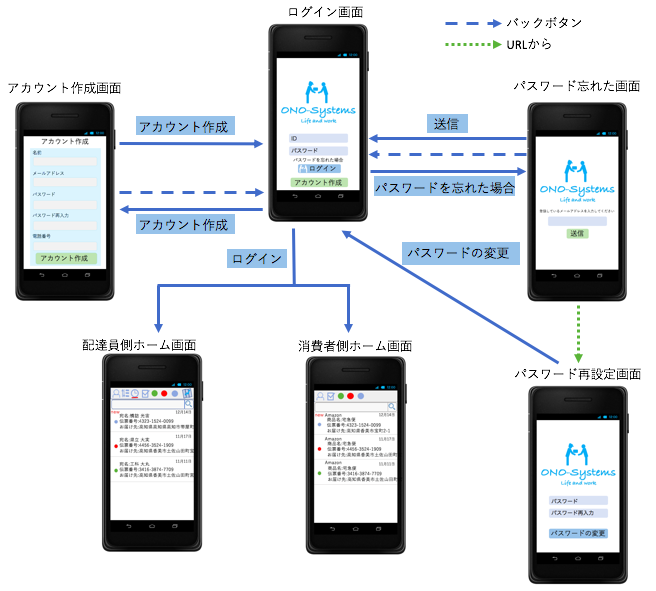
\includegraphics[width=150mm]{screen_transition_login.png}
  \caption{ログイン画面からの画面遷移図}
  \label{fig:login}
 \end{center}
\end{figure}
\begin{figure}[H]
 \begin{center}
  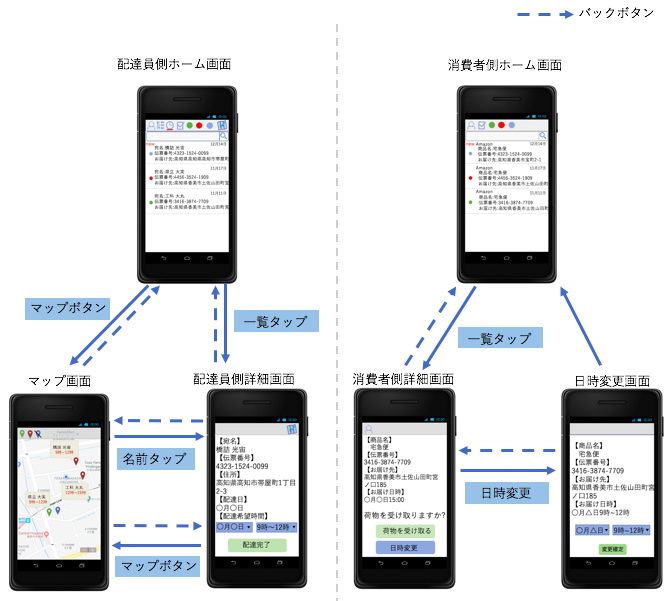
\includegraphics[width=150mm]{screen_transition_home.png}
  \caption{ホーム画面からの画面遷移図(左:配達員側,右:消費者側)}
  \label{fig:home}
 \end{center}
\end{figure}
\subsection{モジュール仕様}
Androidの各モジュールの仕様は以下の通りです.

\subsubsection{MainActivityクラス}
起動時に呼び出さるクラスで,画面遷移のルートを担います.
MainActivityクラスのモジュールは以下の通りであす.

\begin{itemize}
\item createLoginActivity()\\
動作: ログイン画面に遷移する.ログイン画面を生成したときに,loginCallbackの参照を渡す.\\
引数: なし\\
返り値: なし

\item createHomeActivity()\\
動作: ホーム画面に遷移する.ホーム画面を生成したときに,sessionIdも渡す.\\
引数: sessionId, userType\\
返り値: なし

\item loginCallback()\\
動作: ログインに成功したときに呼び出され,ホーム画面の生成を呼び出す.\\
引数: int sessionId, int userType\\
返り値: なし
\end{itemize}

\subsubsection{Requestクラス}
サーバにリクエストを投げる際に使用するクラスです.
\begin{itemize}
\item setSessionId()\\
動作: セッションIDを設定するstaticメソッド.\\
引数: sessionId\\
返り値: なし

\item sendRequest()\\
動作: サーバにリクエストを投げる.bodyはjsonでわたす.セッションIDがあれば付与してリクエストする.返り値はResponseDataクラスのオブジェクト.\\
引数: URL, json\\
返り値: ResponseData
\end{itemize}

\subsubsection{ResponseDataクラス}
ResponseDataで定義する要素を,表\ref{responseTable}に示します.\\
\begin{table}[htb]
\centering
\caption{ResponseDataクラスで定義する変数}
\label{responseTable}
\begin{tabular}{|ll|}
\hline
型 & 変数名       \\ \hline
String & json  \\
int &  statusCode\\
String & status  \\\hline
\end{tabular}
\end{table}

\subsubsection{LoginActivityクラス}
ログイン画面を定義するクラスで,ログイン機能を実現します.
このクラスでは,MainActivityの関数呼び出しを行うため,インタフェースの定義を行います.
LoginActivityクラスのメソッドは以下の通りであす.
\begin{itemize}
\item  interface LoginCallback \\
  動作: コールバック関数である,loginCallbackを定義する.\\
    引数: なし\\
    返り値: なし

  \item loginCallback(Connection connection)\\
    動作: MainクラスのloginCallback メソッドを定義する.\\
    引数: connection\\
    返り値: なし

  
  \item setCallback(LoginCallback callback)\\
  動作:  定義したcallbackに,引数として渡されたcallbackを設定する.\\
  引数:  callback\\
  返り値: なし

  \item login()\\
  動作:  アクティビティの生成完了後,端末内に保持されているユーザIDとパスワードをサーバに送信し,ログインを試みる.\\
  引数: なし\\
  返り値: なし
  
\item loginButton()\\
動作:  ログインボタンが押された際にloginを呼び出す.\\
  引数:  view\\
  返り値: なし

\item login(int user\verb|_|id, string password)\\
  動作:  サーバにユーザIDとパスワードを送信し,ログインを試行する.\\
  (入力) user\verb|_|id,password\\
  返り値: なし

  \item sendToken(User.token token)\\
  動作:  自分のトークンをサーバに送信する.\\
  引数:  token\\
  返り値: なし
  
  \item sendNoticeToken()\\
  動作:  通知を送ってもらうために,サーバにトークンを送信する.\\
  引数: なし\\
  返り値: なし

  \item transitionActivity(Connection connection)\\
  動作:  ログインに成功した場合,コールバック関数を呼び出す.\\
  引数:  connection\\
  返り値: なし

  \item createNewAccountActivity()\\
  動作:  ログイン画面のアカウント作成ボタンが押された際,アカウント作成画面へ遷移する.\\
  引数:  なし\\
  返り値: なし
\end{itemize}


\subsubsection{NewAccountActivityクラス}
アカウント作成画面を定義するクラスで,新規アカウント作成機能を実現します.
\begin{itemize}
  \item createNewAccountButton()\\
動作:  アカウント作成画面のアカウント作成ボタンが押された際 createNewAccount を呼び出す.アカウント作成終了後,ログイン画面に戻る.\\
  引数:  view\\
  返り値: なし

 \item createNewAccount()\\
  動作:  入力されたデータで新規アカウントの作成を行う.\\
  引数:  name,mail,tel,address,password\\
  返り値: なし
\end{itemize}

\subsubsection{HomeActivityクラス}
ホーム画面を定義する継承元のクラスで,消費者側・配達員側の共通機能を実装します.
ホーム画面は,配達物の一覧を表示する画面です.
配達物の受取可否のステータス別に表示する機能や検索機能,プロフィール情報変更機能を実現します.
消費者側・配達員側の非共通機能はこのクラスを継承し,それぞれのクラスで実装します.
HomeActivityクラスのメソッドは以下の通りです.
\begin{itemize}
\item reloadDeliveries()\\
  動作: deliveriesInfoから配達物一覧を表示する.deliveriesInfoはgetDeliveriesメソッドから取得する.\\
  引数: なし\\
  返り値: なし

  \item getDeliveries()\\
   配達物一覧の取得を行うabstractメソッド\\

  \item editProfile()\\
   プロフィール情報の編集を行うためのabstractメソッド\\

  \item updateProfile()\\
    プロフィール情報を更新するabstractメソッド\\

  \item findDeliveryButton()\\
  動作:  検索窓に入力された内容に該当する配達物を表示させるボタン.押されたらfindDeliveriesメソッドを呼び出す.また,refleshメソッドを呼び出し更新する.\\
  引数:  view\\
  返り値:  なし

  \item findDeliveries()\\
  動作:  検索窓に入力された情報と一致するdeliveriesInfo(ship\verb|_|from)のvisibleをtrueにする\\
  引数:  検索窓に入力された情報\\
  返り値:  なし
 
  \item reflesh()\\
  動作:  ホーム画面を再描画する.指定した間隔でreloadDeliveriesメソッド呼び出す.\\
  引数:  なし\\
  返り値:  なし

  \item editProfileButton()\\
  動作:  Profile編集画面を出すためのボタン.押されたらeditProfileメソッド呼び出す.\\
  引数:  view\\
  返り値:  なし

  \item receivableSelectButton()\\
  動作:  受取可否のステータス別に表示するボタン.viewからどのボタンが押されたかを判定し,toggleVisibleFromReceivableメソッドを呼び出す\\
  引数:  view\\
  返り値:  なし

  \item toggleVisibleFromReceivable()\\
  動作:  該当ステータスの表示非表示を切り替え,refleshメソッドを呼び出し再描画する.\\
  引数:  status\\
  返り値:  なし

  \item showDeliveryDetailActivity()\\
  動作:  配達物詳細画面へ遷移する.\\
  引数:  deliveriesInfo\\
  返り値:  なし
\end{itemize}

\subsubsection{Deliveryクラス}
配達物に関する情報を持つクラスです.
Deliveryクラスで定義する要素を,表\ref{deliveryTable}に示します.\\
\begin{table}[htb]
\centering
\caption{Deliveryクラス}
\label{deliveryTable}
\begin{tabular}{|llc|}
\hline
型 & 変数名 & 状態      \\ \hline
string  & name  &      \\
string & address &      \\
long  &  slip\verb|_|number  &    \\
long & ship\verb|_|from &      \\
int & time &      \\
int & receivable\verb|_|status &     \\
int & delivered\verb|_|status  &    \\
boolean & visible  &  true:表示,false:非表示    \\
int & DELIVERED  &  1  \\
int & UNDELIVERED  & 0   \\
int & UNSELECTED  &  0  \\
int & UNRECEIVABLE  & 1   \\
int & RECEIVABLE  & 2   \\\hline
\end{tabular}
\end{table}

\subsubsection{CustomerHomeActivityクラス}
消費者側のホーム画面を定義するクラスで,HomeActivityクラスを継承して実装します.
CustomerHomeActivityクラスのメソッドは以下の通りです.
  \begin{itemize}
  \item getDeliveries()\\
  動作:  消費者IDを用いてデータベースから配達物一覧の取得を行う.\\
  引数:  customer\verb|_|id\\
  返り値:  deliveriesInfo(slip\verb|_|number, name, address, time, derivered\verb|_|status, receive\verb|_|status)

  \item editProfile()\\
  動作:  userEntityから引数を取得する.また,getProfileCustomerとupdateProfileのメソッドを呼び出して変更を行う.\\
  引数:  userEntity\\
  返り値:  なし

  \item getProfileCustomer()\\
  動作:  消費者IDを利用してデータベースからプロフィール情報を取得する.\\
  引数:  customer\verb|_|id\\
  返り値:  userEntity(name, mail, tel, address)

  \item updateProfile()\\
  動作:  データベース上で消費者の情報を更新する.\\
  引数:  userEntity\\
  返り値:  なし
\end{itemize}

\subsubsection{CourierHomeActivityクラス}
配達員側のホーム画面を定義するクラスで,HomeActivityクラスを継承します.
配達物の一覧を時間順や距離順でソートする機能を持ちます.
配達員側の画面では,マップ画面に遷移することができます.
CourierHomeActivityクラスのメソッドは以下の通りです.
\begin{itemize}
  \item editProfile()
  動作:  userEntityから引数を取得する.また,getProfileCourierとupdateProfileのメソッドを呼び出して変更を行う.\\
  引数:  userEntity\\
  返り値:  なし

  \item getProfileCourier()
  動作:  配達員IDを利用してデータベースからプロフィール情報を取得する.\\
  引数:  driver\verb|_|id\\
  返り値:  userEntity(name, mail, tel, store\verb|_|code)

  \item updateProfile()\\
  動作:  データベース上で配達員の情報を更新する\\
  引数:  userEntity\\
  返り値:  なし

  \item getDeliveries()\\
  動作:  配達員IDを用いてデータベースから配達物一覧の取得を行う.\\
  引数:  driver\verb|_|id\\
  返り値:  deliveriesInfo(slip\verb|_|number, name, address, time, derivered\verb|_|status, receive\verb|_|status)

  \item sortTimeButton()\\
  動作:  時間順でソートするためのボタン.ソートする必要があるのか判定した上で,ソートが完了した配列をviewDeliveriesに格納し,refleshメソッドを呼び出す.ソートをするためにsortTimeメソッドを呼び出す.\\
  引数:  view\\
  返り値:  なし

  \item sortTime()\\
  動作:  deliveriesInfoから取得したtimeを利用し,時間順に配達物をソートする.\\
  引数:  deliveriesInfo(time)\\
  返り値:  なし

  \item sortDistanceButton()\\
  動作:  距離順でソートするボタン.ソートする必要があるのか判定した上で,ソートが完了した配列をviewDeliveriesに格納し,refleshメソッドを呼び出す.ソートをするためにsortDistanceを呼び出す.\\
  引数:   view\\
  返り値:  なし

  \item sortDistance()\\
  動作:  距離順に配達物をソートする.getMapInfoメソッドを呼び出して商品の宛先情報を取得し,距離を計算する.\\
  引数:  distanceProduct(slip\verb|_|number, lat, lng)\\
  返り値:  なし

  \item getMapInfo()\\
  動作:  slip\verb|_|numberを用いてデータベースから商品の宛先の緯度経度を取得する.\\
  引数:  slip\verb|_|number\\
  返り値:  distanceProduct(slip\verb|_|number, lat, lng)

  \item showMapActivity()\\
  動作:  マップ画面へ遷移する.\\
  引数:  deliveriesInfo\\
  返り値:  なし
\end{itemize}

\subsubsection{DeliveryDetailクラス}
配達物詳細画面を定義する継承元のクラスで,消費者側・配達員側の共通機能を実装します.
荷物情報の詳細を表示する画面です.
 消費者側・配達員側の非共通機能はそれぞれのクラスで実装します.
 
\begin{itemize}
 \item reschedulingButton()\\
 配達日時の変更ボタンを押したときに発火されるabstractメソッド.\\
\end{itemize}

\subsubsection{CustomerDeliveryDetailクラス}
消費者側の配達物詳細画面のクラス.DeliveryDetailクラスを継承します.
荷物受取可否を選択する機能を実現します.
CustomerDeliveryDetailクラスのメソッドは以下の通りです.
\begin{itemize}
 \item reschedulingButton()\\
 動作: 日時変更画面へ遷移する\\
 引数: delivery\\
 返り値: なし

 \item receivableButton()\\
 動作: 荷物を受け取るボタンを押したときに発火されるメソッド.荷物を受け取れる旨をサーバに送信する.\\
 引数: なし\\
 返り値: なし
\end{itemize}

\subsubsection{CourierDeliveryDetailクラス}
配達員側の配達物詳細画面を定義するクラスで,DeliveryDetailクラスを継承します.
配達完了を報告する機能を実装します.
CourierDeliveryDetailクラスのメソッドは以下の通りです.
\begin{itemize}
\item reschedulingButton()\\
 動作: 日時変更画面へ遷移する.\\
 引数: なし\\
 返り値: なし

\item deliveredButton()\\
 動作: 配達完了ボタンを押したときに発火されるメソッド.配達完了の旨をサーバに送信する.\\
 引数: なし\\
 返り値: なし
\end{itemize}

\subsubsection{TimeChangeクラス}
 日時変更画面のクラスで,配達日時の変更を確定する機能を持ちます.
\begin{itemize}
 \item CreateTimeChange()\\
   動作: 変更確定ボタンを押したときに発火されるメソッド.日時の変更を確定する.変更内容をサーバに送信する.\\
 引数: なし\\
 返り値: なし
\end{itemize}

\subsubsection{CourierMapActivityクラス}
マップ画面を定義するクラスで,配達員側だけが遷移できる画面です.
ピンの位置で配達先の住所を表示する機能や,受取可否ステータス別の絞り込み表示機能を実現します.
CourierMapActivityクラスのメソッドは以下の通りです.
\begin{itemize}
\item setDeliveries()\\
  動作: データベースに配達物のリストを要求し格納する.\\
引数: なし\\
返り値: なし

\item refineDeliveriesButton()\\
動作: 荷物情報のrecievableを見て絞りこみ条件に一致するもののvisibleをtrueにさせ,それ以外をfalseにする.\\
引数: なし\\
返り値: なし

\item showDeliveryDetailActivity()\\
動作: マップ画面から配達物詳細画面へ遷移する.\\
引数: delivery\\
返り値: なし

\item reflesh()\\
動作: 画面の再描画\\
引数: 配達物のリスト,絞り込み条件\\
返り値: なし
\end{itemize}

\section{Server モジュール設計}
Serverのモジュール設計を以下に示します.
Serverモジュールの引数や返り値で使用している単語は,表\ref{serverTable}の通りです.
\begin{table}[htb]
\centering
\caption{本節で使用する変数の定義}
\label{serverTable}
\begin{tabular}{|lll|}
\hline
型 & 変数名 & 意味      \\ \hline
int & driver\verb|_|id & 配達員のID     \\
int & costomer\verb|_|id & 消費者のID     \\
int & manager\verb|_|id & 管理者のID     \\
string  & name  & 名前     \\
string & possword & パスワード     \\
string & mail & メールアドレス     \\
string & tel & 電話番号     \\
string & address & 住所     \\
long  &  slip\verb|_|number  & 伝票番号   \\
long & ship\verb|_|from & 発送元     \\
int & time & 配達日・時間     \\
int & receivable\verb|_|status & 配達状況    \\
int & delivered\verb|_|status  &  受け取り可否  \\
string & token & 端末登録トークン \\ \hline
\end{tabular}
\end{table}
receivable\verb|_|statusは,未配達を0,配達済みを1で表します.
delivered\verb|_|statusは,未選択の状態を0,受け取れない場合は1,受け取れる場合は2で状態を表現します.

\subsection{モジュール構成}
サーバは,認証,配達員側,消費者側のモジュールに加え,管理者側や通知機能に関するモジュールから構成されています.

\subsection{モジュール仕様}
Serverの各モジュールの仕様は以下の通りです.
\subsubsection{認証機能}
ログインを行う際に使用する認証系のモジュールについて示します.
ログイン機能では,配達員側,消費者側どちらも同じモジュールを用いて認証を行います.
\begin{itemize}
\item Login.java\\
  動作: 初めにハッシュ値を計算しているか確認を行う.計算していなければパスワードからハッシュ値の計算を行いデータベースに値を格納する.次に,IDとパスワードからデータベースにあるハッシュ値を比較し,ログイン処理を行う.最後に,セッション情報をサーバ内に記憶させる.\\
  引数: id,password\\
  返り値: customer\verb|_|id,driver\verb|_|id,manager\verb|_|id のいずれか一つ(NULL値なら認証不可)
\item AuthFilter.java\\
  動作: 認証が通っているかの判別を各サーブレットについて行う.判別にはセッション情報を用いる.このプログラムは,認証が必要な全てのサーブレットに対して行う.\\
  引数: なし\\
  返り値: なし
\item RegisterAccount.java\\
  動作: 入力された情報からデータベースに新たな消費者の登録を行う.また,パスワードからハッシュ値を計算しデータベース内に格納する.\\
  引数: name,mail,password,tel,address\\
  返り値: なし
\end{itemize}

\subsubsection{配達員側}
配達員側のモジュールを以下に示します.
\begin{itemize}
\item TopCourier.java\\
  動作: 当日に配達する荷物情報を,データベースからドライバーIDを参照して送信する.\\
  引数: driver\verb|_|id\\
  返り値: name,slip\verb|_|number,ship\verb|_|from,address,time,receivable\verb|_|status,delivered\verb|_|status
\item SettingCourier.java\\
  動作: 配達員が入力した情報からデータベース内の配達員情報の変更を行う.\\
  引数: (配達員の)name,mail,password,tel\\
  返り値: なし
\item ChangeTimeCourier.java\\
  動作: 入力された情報からデータベース内の配達希望日時の変更を行う.\\
  引数: slip\verb|_|number,time\\
  返り値: time
\item CompleteCourier.java\\
  動作: 伝票番号からデータベース内の荷物情報に配達済みのフラグを立てる.\\
  引数: slip\verb|_|number\\
  返り値: なし
\item  InformationCourier.java\\
 動作: データベースから配達員の情報を取得し,送信する.\\
 引数: driver\verb|_|id\\
返り値: name,mail,tel
\end{itemize}

\subsubsection{消費者側}
消費者側のモジュールを以下に示します.
\begin{itemize}
\item TopCustomer.java\\
  動作: 入力された情報から利用者の荷物情報を送信する.\\
  引数: customer\verb|_|id\\
  返り値: name,slip\verb|_|number,ship\verb|_|from,address,time,receivable\verb|_|status,delivered\verb|_|status
\item SettingCustomer.java\\
  動作: 入力された情報からデータベース内の消費者情報の変更を行う.\\
  引数: (消費者の)name,mail,password,tel,address\\
  返り値: なし
\item ReceiveCustomer.java\\
  動作: 伝票番号から荷物受け取りの可否をデータベース内に格納する.\\
  引数: slip\verb|_|number\\
  返り値: なし
\item ChangeTimeCustomer.java\\
  動作: 消費者が入力した情報からデータベース内の配達希望日時の変更を行う.\\
  引数: slip\verb|_|number,time\\
  返り値: time
  \item InformationCustomer.java\\
 動作: データベースから利用者の情報を取得し,送信する.\\
 引数: customer\verb|_|id\\
返り値: name,mail,tel,address
\end{itemize}

\subsubsection{通知機能}
通知機能のモジュールを以下に示します.
\begin{itemize}
\item Notification.java\\
  動作: トークンを受け取り,通知を送ってもらうようFirebaseに対してデータを送信する.\\
  引数: token\\
  返り値: token,テキスト内容
\end{itemize}

\subsubsection{管理者側}
管理者側のモジュールを以下に示します.
\begin{itemize}
\item LoginManager.jsp\\
  動作: 管理者ページへのログインを行う.\\
  引数: manager\verb|_|id,password\\
  返り値: なし
\end{itemize}


\section{データベース設計}
本システムではデータベースにAWS(AmazonWebService)を使用します.\\
実体関連を表したER図を,図\ref{fig:erd}に示します.
PKは主キー,MKは外部キーを表しています.
\begin{figure}[H]
 \begin{center}
  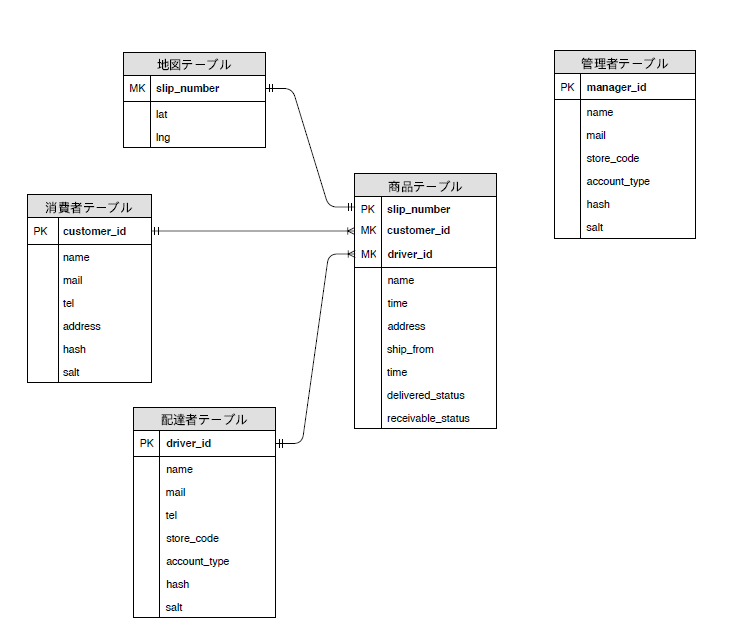
\includegraphics[width=150mm]{erd.png}
  \caption{実体関連図}
  \label{fig:erd}
 \end{center}
\end{figure}
 
\subsection{各テーブルの詳細}
本システムのデータベースには,5個のデータテーブルを用います.各データテーブルの役割と属性を以下に示します.
\subsubsection{消費者テーブル}
消費者テーブルでは,消費者に関する情報を管理します.このテーブルのデータテーブルを表\ref{customer}に示します.
\begin{table}[htb]
  \caption{消費者テーブル}
  \label{customer}
  \begin{center}
    \begin{tabular}{|c|c|c|c|c|c|} \hline
      属性 & データ型/長 & NULL & Key & 初期値 & その他 \\ \hline \hline
      customer\verb|_|id & int(9) unsigned & NO & PRIMARY & NULL & auto\verb|_|increment\\ \hline
      name & varchar(64) & NO &   &  & \\ \hline
      mail & varchar(64) & NO &   &  & \\ \hline
      tel & varchar(11) & YES &   & NULL & \\ \hline
      address & varchar(128) & YES &   & NULL & \\ \hline
      hash & varchar(255) & NO &   &  & \\ \hline
      salt & varchar(255) & NO &   &  & \\ \hline
    \end{tabular}
  \end{center}
\end{table}

\subsubsection{配達員テーブル}
配達員テーブルでは,配達員に関する情報を管理します.このテーブルのデータテーブルを表\ref{driver}に示します.
\begin{table}[htb]
  \caption{配達員テーブル}
  \label{driver}
  \begin{center}
    \begin{tabular}{|c|c|c|c|c|c|} \hline
      属性 & データ型/長 & NULL & Key & 初期値 & その他 \\ \hline \hline
      driver\verb|_|id & int(9) unsigned & NO & PRIMARY & NULL & auto\verb|_|increment\\ \hline
      name & varchar(64) & NO &   &  & \\ \hline
      mail & varchar(64) & NO &  &  & \\ \hline
      tel & varchar(11) & YES &  & NULL & \\ \hline
      store\verb|_|code & varchar(64) & YES &   & NULL & \\ \hline
      account\verb|_|type & int(1) unsigned & YES &   & NULL & \\ \hline
      hash & varchar(255) & NO &   &  & \\ \hline
      salt & varchar(255) & NO &   &  & \\ \hline
    \end{tabular}
  \end{center}
\end{table}

\subsubsection{商品テーブル}
商品テーブルでは,商品に関する情報を管理します.このテーブルのデータテーブルを表\ref{delivery}に示します.
\begin{table}[htb]
  \caption{商品テーブル}
  \label{delivery}
  \begin{center}
    \begin{tabular}{|c|c|c|c|c|c|} \hline
      属性 & データ型/長 & NULL & Key & 初期値 & その他 \\ \hline \hline
      slip\verb|_|number & varchar(12) & NO & PRIMARY & NULL & \\ \hline
      name & varchar(64) & NO &   &  & \\ \hline
      address & varchar(128) & NO &   &  & \\ \hline
      ship\verb|_|from & varchar(64) & YES &  & NULL & \\ \hline
      time & varchar(10) & YES &   & NULL & \\ \hline
      delivered\verb|_|status & int(1) unsigned & NO &   & 0 & \\ \hline
      receivable\verb|_|status & int(1) unsigned & NO &  & 0 & \\ \hline
      customer\verb|_|id & int(9) unsigned & NO & MULTIPLE & NULL & \\ \hline
      driver\verb|_|id & int(9) unsigned & NO & MULTIPLE & NULL & \\ \hline
    \end{tabular}
  \end{center}
\end{table}

\subsubsection{管理者テーブル}
管理者テーブルでは,管理者に関する情報を管理します.このテーブルのデータテーブルを表\ref{manager}に示します.
\begin{table}[htb]
  \caption{管理者テーブル}
  \label{manager}
  \begin{center}
    \begin{tabular}{|c|c|c|c|c|c|} \hline
      属性 & データ型/長 & NULL & Key & 初期値 & その他 \\ \hline \hline
      manager\verb|_|id & int(1) unsigned & NO & PRIMARY & NULL & auto\verb|_|increment\\ \hline
      name & varchar(64) & NO &   &  & \\ \hline
      mail & varchar(64) & NO &  &  & \\ \hline
      store\verb|_|code & varchar(64) & YES &   & NULL & \\ \hline
      account\verb|_|type & int(1) unsigned & YES &   & NULL & \\ \hline
      hash & varchar(255) & NO &   &  & \\ \hline
      salt & varchar(255) & NO &   &  & \\ \hline
    \end{tabular}
  \end{center}
\end{table}

\subsubsection{地図テーブル}
地図テーブルでは,地図に関する情報を管理します.このテーブルのデータテーブルを表\ref{map}に示します.
\begin{table}[htb]
  \caption{地図テーブル}
  \label{map}
  \begin{center}
    \begin{tabular}{|c|c|c|c|c|c|} \hline
      属性 & データ型/長 & NULL & Key & 初期値 & その他 \\ \hline \hline
      slip\verb|_|number & varchar(12) & NO & MULTIPLE & NULL & auto\verb|_|increment\\ \hline
      lat & double(8,6) & YES &   & NULL & \\ \hline
      lng & double(9,6) & YES &   & NULL & \\ \hline
    \end{tabular}
  \end{center}
\end{table}


\section{バージョン管理規約}
本システムの開発では,GitHub を用いてファイルの管理を行います.GitHub を使用する際には,以下の規則を遵守します.
\begin{itemize}
\item ドキュメント関連の資料は,onosystem-doc で管理する
\item Android のソースコードは,onosystem-android で管理する
\item Server のソースコードは,onosystem-server で管理する
\item 編集作業を行う際には,ブランチを切ってコミットする
\item 開発用ブランチの名前は,「dev\verb|_|○○(開発している機能名)」にする
\item 細かい頻度でコミットする(1日の作業ごとに纏めてコミットしない)
\item コミットのコメントはわかりやすい内容にする
\item Pull Requests されたものを確認し,評価をリアクションのアイコンを追加することで示す
\item Pull Requests に対して高評価が3つ以上ある場合には master に Merge する
\end{itemize}

\end{document}
